% TODO:
%   - Kijk na of titels in header overflowen
% ----------  
% Questions:
%   - XXX

% https://www.brainlatam.com/blog/wet-dry-active-and-passive-electrodes.-what-are-they-and-what-to-choose-413

% https://www.brainlatam.com/blog/a-brief-introduction-to-eeg-and-the-types-of-electrodes-75

% https://iopscience.iop.org/article/10.1088/1741-2552/abc902/pdf

% bci_review_book_chapter

% In a new chapter, reset the GLS to once again use full version in first occurence
\glsresetall

\chapter{Origins and acquisition of biomedical signals}
\label{ch:biomedical_signals}

% ---------------------------------------------- 
% INTRODUCTION
% ---------------------------------------------- 
\section{Introduction to this chapter}
\label{sec:biomedical_signals_introduction}
% NOTE: "Introduction" exists in each chapter and gives short intro to chapter + what can be expected in chapter

Whilst Chapter \ref{ch:bci} has provided an in-depth intuitive introduction to \glspl{bci}, some more technical aspects need addressing as well to provide a computer scientist with all of the required foundational knowledge for \gls{bci} research.
This chapter provides the required technical knowledge on the data that \gls{bci} systems use, brain signals.
Brain signals are only one of the many types of \gls{biosignal} present in the human body.
Whilst from a computer scientist's perspective brain signals may just be another type of input data to a classification model, having at least a basic understanding of this data is crucial in making good classification algorithms for \gls{bci} systems.
Even when using \gls{dl} approaches where no manual feature engineering has to be done and where basic models without much thought may have pleasing results, understanding the data will allow for the creation of better models.
This understanding of the data also helps in troubleshooting why some models may not have the desired results.

To provide this basic understanding, this chapter starts by briefly discussing \glspl{biosignal} in general.
It is discussed what \glspl{biosignal} are and where they originate from in the human body.
After this general discussion on \glspl{biosignal}, a focus is put on the different \glspl{biosignal} from the human brain, with brain signals measured using \gls{eeg} in particular.
This \gls{eeg} measuring technique and other measuring techniques are also discussed in greater detail.
Whilst it is addressed that \gls{eeg} has some fundamental shortcomings over other measuring modalities, it also has some attractive properties over these alternatives.
These attractive properties are listed and provide an argument as to why the remainder of this master thesis will focus on \gls{eeg} and \gls{mi} \gls{eeg} in particular.

% ---------------------------------------------- 
% ORIGINS
% ---------------------------------------------- 

\section{Biosignals in the human body}
\label{sec:biomedical_signals_biosignals_in_human}

In theory, a \glspl{biosignal} is nothing more than a measurement over time of a living
being.
In practice, these \glspl{biosignal} are closely related to physiological processes.
This makes it possible to monitor or detect those physiological processes using \glspl{biosignal}.
\Glspl{biosignal} can be produced by different energy forms, such as the electrical energy form when measuring \gls{eeg} in \gls{mv}.
Table \ref{tab:biomedical_signals_energy_forms} summarizes some of these energy forms and which type of \glspl{biosignal} they can produce.
Whilst living beings, including humans, produce many different types of \glspl{biosignal}, this master thesis will only consider time-varying electrical \glspl{biosignal}.
These types of \glspl{biosignal}, sometimes reffered to as \gls{elecbiosignal}, are the ones used as input data for \gls{bci} systems.
\Citet{biosignal_definition} discusses these and other types of \glspl{biosignal} in greater detail.

\begingroup
\setlength{\tabcolsep}{6pt} % Default value: 6pt
\renewcommand{\arraystretch}{2} % Default value: 1
\begin{table}[]
    \resizebox{\columnwidth}{!}{%
    \begin{tabular}{|l|p{5cm}|p{7cm}|}
        \hline
        \textbf{Energy form} & \textbf{Variable type}                 & \textbf{Biosignals}                                                                     \\ \hline
        Chemical             & Chemical activity and/or \newline concentration & Blood ions, O2, CO2, pH, hormonal \newline concentrations, and other chemistry                             \\ \hline
        Mechanical           & Position, force, torque or \newline pressure    & Muscle movement or cardiovascular pressures, muscle contractility, valve and other cardiac sounds \\ \hline
        Electrical           & Voltage or current                     & EEG, ECoG, ECG, EMG, EOG, ERG, EGG, GSR and EDA                                                                 \\ \hline
        Thermal             & Temperature                            & Body temperature and thermography                                                                    \\ \hline
        \end{tabular}%
        }
    \captionsetup{width=0.8\linewidth}
    \captionsetup{justification=centering}
    \caption{Some of the different energy forms in living beings and the most important measurable biosignals they produce. Data from \citet{biosignal_definition}.}
    \label{tab:biomedical_signals_energy_forms}
\end{table}
\endgroup

% - - - - - - - - - -
% how produced
% - - - - - - - - - -

\subsection{Origin of electricity inside the the human body}
\label{subsec:biomedical_signals_biosignals_electrical}

Electricity in the human body, better known as bioelectricity, can be seen as the generation or action of tiny electric currents and voltages in physiological processes.
As shown in Table \ref{tab:biomedical_signals_energy_forms}, the measurement of this bioelectricity is what enables the monitoring of \glspl{elecbiosignal}.
This is one of the reasons \glspl{biosignal} are closely related to physiological processes since it measures the bioelectricity used in some of these processes.
A complete understanding of how bioelectricity is made, maintained and transmitted in the human body isn't required for a computer scientist to contribute to the \gls{bci} field.
However, a superficial understanding of this process makes it easier to understand the limits of the accompanied \glspl{elecbiosignal}.
For this reason, the remainder of this section gives a simplified explanation of how bioelectricity is made, maintained and transmitted in the human brain.
This explanation is based on chapter 12 of the recently renewed book by \citet{bioelec_book}, an \gls{eeg} focused explanation of bioelectricity by \citet{eeg_bioelec_creation} and multiple YouTube videos by Neuroscientifically Challenged\footnote{\url{https://youtu.be/tIzF2tWy6KI}}\footnote{\url{https://youtu.be/W2hHt_PXe5o}}\footnote{\url{https://youtu.be/WhowH0kb7n0}}.

% | | | | | | | | | | | | |

\subsubsection{Resting membrane potential causes negatively charged neurons}
\label{subsubsec:biomedical_signals_biosignals_electrical_membrane_potential}

As was already addressed in Section \ref{subsec:bci_gaining_popularity_better_measuring}, the human brain has billions of neurons with \citet{neurons_book} stating that around $10^7$ parallel pyramidal neurons reside in only a single $cm^3$ of the brain cortex alone.
A neuron, also known as a nerve cell, is an electrically excitable cell.
Being an electrically excitable cell, a neuron has a resting membrane potential.
This resting membrane potential is around $-70$ \gls{milv} and expresses the difference in electrical charge between the inside and the outside of a neuron.
This negative difference is maintained by the sodium-potassium pump which is responsible for the hydrolysis of ATP to ADP.
During this hydrolysis process the sodium-potassium pump releases three positively charged sodium ions ($Na^+$) whilst only taking in two positively charged potassium ions ($Ka^+$), this difference causes the membrane potential to remain negative.

% | | | | | | | | | | | | |

\subsubsection{Action potential allows for neuron communication}
\label{subsubsec:biomedical_signals_biosignals_electrical_action_potential}

Whilst the sodium-potassium pump inside the neuron explains why there is a negative resting membrane potential of around $-70$ \gls{milv}, it doesn't explain the variable volt measurements of \gls{eeg}.
The change in membrane potential occurs when the neuron gets excited.
The most common way a cell gets excited is through the process known as an action potential.
An action potential forms the basis for electrical signalling within neurons, enabling some form of communication between them.
To do this communication, neurotransmitters released by another neuron bind to receptors on the dendrites of the receiving neuron which has a depolarization effect.

This depolarization causes the neuron to become less polarized, resulting in its membrane potential moving close to zero.
When sufficient depolarization occurs, the action potential process could start.
This process is visualised in Figure \ref{fig:biomedical_signals_action_potential}.
For the action potential process to start, the depolarization should be of such a magnitude that the neuron reaches its threshold membrane potential, which is around $-55$ \gls{milv}.
This is achieved through the repeated binding of neurotransmitters to the receptors.
The annotation for "failed initiations" in Figure \ref{fig:biomedical_signals_action_potential} denotes the common situations when the threshold membrane potential is not reached.

When the threshold is reached, a large number of sodium channels open, allowing many positive sodium ions ($Na^+$) into the neuron, causing the membrane potential to rise quickly.
This depolarization is what creates the electrical signal known as the action potential that travels down the neuron to eventually release neurotransmitters itself.
Eventually, a peak is reached, after which the sodium channels close, not allowing any further sodium ions ($Na^+$) to enter the neuron.
To return to its resting membrane potential, the neuron opens its potassium channels to release many potassium ions ($Ka^+$).
This is known as the falling phase where the neuron repolarizes.
However, the release of positive potassium ions ($Ka^+$) happens so quickly that the membrane potential falls below the resting membrane potential.
The neuron is now hyperpolarized, denoted as undershoot in Figure \ref{fig:biomedical_signals_action_potential}.
During this hyperpolarized state, also known as the refractory period, failed initiations occur more often as it is very difficult to fire the neuron again.
Eventually, the resting membrane potential is reached again and the neuron functions like before.


\begin{figure}[ht]
    \centering
    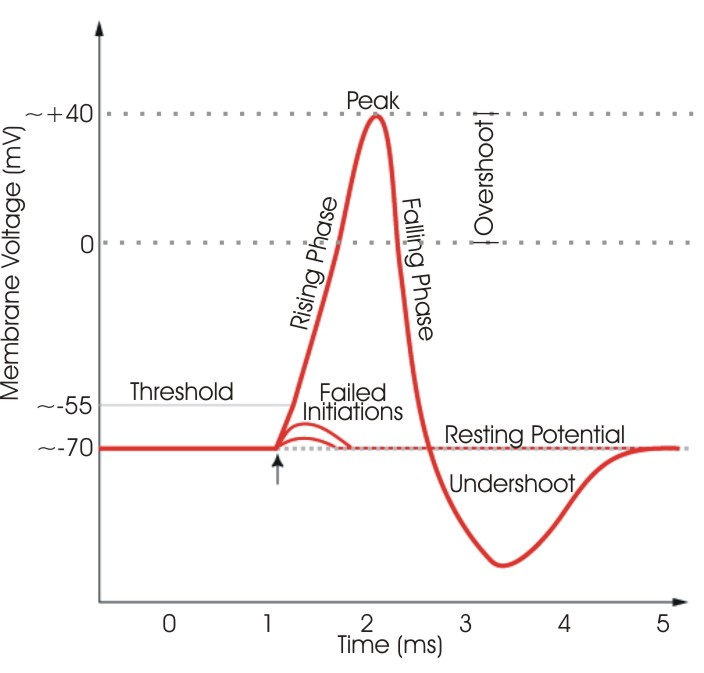
\includegraphics[width=0.7\linewidth]{../images/biosignals/action_potential.jpg}
    \captionsetup{width=0.7\linewidth}
    \captionsetup{justification=centering}
    \caption{Chart of the membrane potential during the action potential process in a neuron. Figure from Synaptidude, GFDL 1.2, via Wikimedia Commons.} 
    \label{fig:biomedical_signals_action_potential}
\end{figure}



% | | | | | | | | | | | | |

\subsubsection{EEG measures postsynaptic potentials}
\label{subsubsec:biomedical_signals_biosignals_electrical_postsynaptic_potential}

Whilst the action potential explains how most changes in membrane potential of an individual neuron occur, it is highly unlikely to be measured by \gls{eeg} and other measuring modalities.
This follows from the fact that, as discussed earlier, many billion neurons make up the brain making it impossible to monitor a singular neuron.
Since action potentials are such rapid current flows, it is highly unlikely enough neighbouring neurons will have an action potential at the same time resulting in a measurable signal.
However, whilst it was discussed how neurotransmitters can cause depolarization which can initialize action potentials, these neurotransmitters can also influence the membrane potential in the opposite direction by causing further polarization.
The release of these neurotransmitters and the binding to the receiving neuron also causes currents known as postsynaptic potentials.
Whilst these are not action potentials, they are essentially what causes an action potential to take place and the action potential can also cause the release of neurotransmitters.
These postsynaptic potentials are present for a longer period than action potentials.
Thus, it is more likely for many neighbouring neurons to have active postsynaptic potentials simultaneously.
The summation of these postsynaptic potential currents from many millions of neurons is what is detected by \gls{eeg}.
However, neurons experiencing action potential at that same time are among many other things sources of noise in this summation of these currents.
\Citet{what_eeg_is_and_measures} explain in greater detail what exactly is measured with \gls{eeg}.



% | | | | | | | | | | | | |

\subsubsection{Biosignals originating from bioelectricity in the human body}
\label{subsubsec:biomedical_signals_biosignals_electrical_biosignals}

Both voltage and current can be measured from bioelectricity, providing many different \glspl{biosignal}.
The measurement of voltage originating from the brain, measured in a non-invasive manner with electrodes on the scalp is known as \gls{eeg}.
Likewise, \gls{ecg} revolves around the non-invasive measurement of voltage originating from the heart.
\Gls{eog} and \gls{erg} are techniques used for measuring bioelectricity that originates from the eyes.
Table \ref{tab:biomedical_signals_energy_forms} provides the most important \glspl{biosignal} related to the measurement of bioelectricity.
The most important \gls{elecbiosignal} in BCI research are \gls{eeg} and the invasive alternative \gls{ecog}.


% - - - - - - - - - -
% Other energy forms
% - - - - - - - - - -

\subsection{Other energy forms and their related biosignals}
\label{subsec:biomedical_signals_biosignals_others}

Section \ref{subsec:biomedical_signals_biosignals_electrical} illustrated that bioelectricity is omnipresent in the human body. 
The human nervous system relies on bioelectricity to quickly carry information from the human body to the brain and the other way around.
The process of muscle contraction is started when the discussed action potentials release neurotransmitters from motor neurons to muscle fibres.
As discussed by \citet{bioelectricity_cancer}, bioelectricity can even be \textit{hijacked} as a way of novel medicine and treatment, i.e. for cancer treatment.

However, bioelectricity is only one energy form present in the human body.
As shown in Table \ref{tab:biomedical_signals_energy_forms}, other energy forms provide many other types of \glspl{biosignal}.
Whilst these are of great importance in many fields, \gls{bci} research is mostly interested in brain activity and thus the \glspl{elecbiosignal} \gls{eeg} and \gls{ecog}.
However, as discussed in Section \ref{subsubsec:bci_common_use_cases_improving_existing_system_smart_home}, hybrid systems are being explored which may combine these \glspl{elecbiosignal} with \glspl{biosignal} from other energy forms.
These types of hybrid systems and the other types of \glspl{biosignal} they use fall outside the scope of this master thesis.

% ---------------------------------------------- 
% MEASURING BRAIN SIGNALS
% ---------------------------------------------- 

\section{Measuring biosignals from the brain}
\label{sec:biomedical_signals_measuring_brain}

Neuroimaging is a discipline focused on capturing the anatomy and function of the \gls{cns}, which includes the brain \citep{neuroimaging}.
As such, the modalities for measuring biosignals in the brain are mostly a subcollection of neuroimaging techniques.
Many different types of these modalities exist, both invasive and non-invasive.
There is no singular best measuring modality and often a trade-off has to be made between affordability, the \gls{snr}, the ease-of-use and the risks involved.
Section \ref{subsec:biomedical_signals_measuring_brain_modalities} will discuss these modalities in further detail.
The remainder of this master thesis then focuses on the \gls{eeg} modality as it remains one of the most attractive modalities for \gls{bci} research.



% - - - - - - - - - -
% Measuring modalities
% - - - - - - - - - -

\subsection{Common measuring modalities in BCI systems}
\label{subsec:biomedical_signals_measuring_brain_modalities}

Research by \citet{human_eeg_discovery} is the first in describing the measurement of brain waves from the human brain in a non-invasive manner.
Because of this, the German neuroscientist and psychiatrist Hans Berger is often seen as the inventor of \gls{eeg}.
Whilst he was one of the first to use the term \textit{elektrenkephalogramm}, it was Richard Caton who first described the findings of bioelectricity in brains in general.
He found this phenomenon in animal brains as early as 1875 \citep{first_eeg}.
Since then, the neuroimaging field has been looking for new ways to capture these electrical signals coming from the brain and monitor the anatomy and function of the \gls{cns} in general.
This has caused the introduction of many different measuring modalities, each with its strengths and weaknesses.
However, many of these modalities require bulky equipment which makes them non-portable and thus non-attractive for use in general \gls{bci} systems \citep{modalities_review1}.

Table \ref{tab:biomedical_signals_modalities} provides an overview of the most common measuring modalities considered for use in \gls{bci} applications together with some of their properties.
\Gls{eeg}, \gls{ecog}, intravescular electrodes and \gls{fnirs} seem most probable to be used in \gls{bci} systems for the foreseeable future.
Because of this, this section focuses on these modalities.
Further refinement of other modalities or even new modalities might cause a shift in the modalities used for \glspl{bci}.
This is already visible with the Elon Musk company Neuralink, discussed in Section \ref{subsec:bci_gaining_popularity_better_measuring}, pushing \glspl{bci} to an invasive future away from the now very commonly used non-invasive \gls{eeg} modality.
 



\begingroup
\setlength{\tabcolsep}{6pt} % Default value: 6pt
\renewcommand{\arraystretch}{2} % Default value: 1
\begin{table}[]
    \resizebox{\columnwidth}{!}{%
    \begin{tabular}{|l|l|l|l|l|l|l|l|l|}
        \hline
        \textbf{Modality}          & \textbf{Invasive} & \textbf{Risks} & \textbf{Temporal resolution} & \textbf{Spatial resolution} & \textbf{Affordability} & \textbf{Ease-of-installation} & \textbf{Ease-of-use} & \textbf{Comfort} \\ \hline
        EEG                        & No                & Low            & 50ms                        & 10mm                       & €                      & Good                          & Good                 & Medium           \\ \hline
        ECoG                       & Yes               & High           & 5ms                         & 1mm                        & €€-€€€                 & Poor                          & Good                 & Good             \\ \hline
        Intravescular electrodes    & Yes               & Medium         & 5ms                          & 2.4mm                       & €€-€€€                 & Poor                          & Good                 & Good             \\ \hline
        fNIRS                      & No                & Low            & 1000ms                       & 10mm                        & €-€€€                 & Good                          & Good                 & Medium           \\ \hline
        Implemented microelectrode & Yes               & High           & 3ms                          & 0.05mm - 0.5mm              & €€€                    & Poor                          & Good                 & Good             \\ \hline
        fTCD                       & No                & Low            & 1ms - 5ms                    & 10mm - 30mm                 & €                      & Medium                        & Medium               & Poor             \\ \hline
        \end{tabular}%
        }
    \captionsetup{width=0.9\linewidth}
    \captionsetup{justification=centering}
    \caption{Overview of the most common neuroimaging modalities for use in BCI systems. Data based on \citet{modalities_review1} and \citet{modalities_review2}.}
    \label{tab:biomedical_signals_modalities}
\end{table}
\endgroup


% | | | | | | | | | | | | |

\subsubsection{Electroencephalography (EEG)}
\label{subsubsec:biomedical_signals_measuring_brain_modalities_eeg}

\Glsfirst{eeg} is a non-invasive technique used to measure the electrical activity of the brain, often expressed in \gls{mv} over time.
Electrodes are most commonly placed on the scalp with as main goal to detect the activity of neurons in the cerebral cortex.
The cerebral cortex, better known as grey matter, is the outmost layer of the brain, closest to the electrodes placed on the scalp.
Whilst more inner layers of the brain also produce information-rich \gls{elecbiosignal}, these signals do not reach the scalp in a clear detectable manner for \gls{eeg} to pick up.
As discussed in Section \ref{subsec:biomedical_signals_biosignals_electrical}, \gls{eeg} is not capable of measuring the individual activity of neurons in the cerebral cortex but rather the activity of large groups of neurons that are active at the same time.
Postsynaptic potentials contribute most to these measurements as action potentials are too short in duration.
The location at which electrodes are placed on the scalp often follows specific standards which are further explained in Section \ref{subsec:biomedical_signals_measuring_brain_standards}.
These electrodes can be divided based on whether they are wet or dry, active or passive and whether they are wired or wireless.
The difference between these types has already been covered in Section \ref{subsec:bci_gaining_popularity_better_measuring}.

The output of these electrodes is processed through a differential amplifier which takes two electrical inputs and displays the output as the difference between these inputs.
This means that an \gls{eeg} measurement displayed from one electrode is not absolute but rather the relative difference between that electrode and another.
The selection of the other electrode for passing through the differential amplifier can differ per device through what is known as the montage of the \gls{eeg} device.
The most common montages are common reference, average reference and bipolar.
The common reference montage uses a predefined electrode as a reference electrode and compares each electrical signal from an electrode with it.
Most commonly this reference electrode is placed on the ear as this is least influenced by brain activity.
The average reference montage compares each electrical signal from an electrode with the averaged electrical signal from all electrodes.
The bipolar montage follows a certain scheme of comparing two always differing electrodes with each other.
Most often this is done in a sequence from the front of the scalp to the back of the scalp.
All of these montages are summarized in Figure \ref{fig:biomedical_signals_eeg_montages}.
The output of the differential amplifier is what is known as the \gls{eeg} measurement.

\begin{figure}[ht]
    \centering
    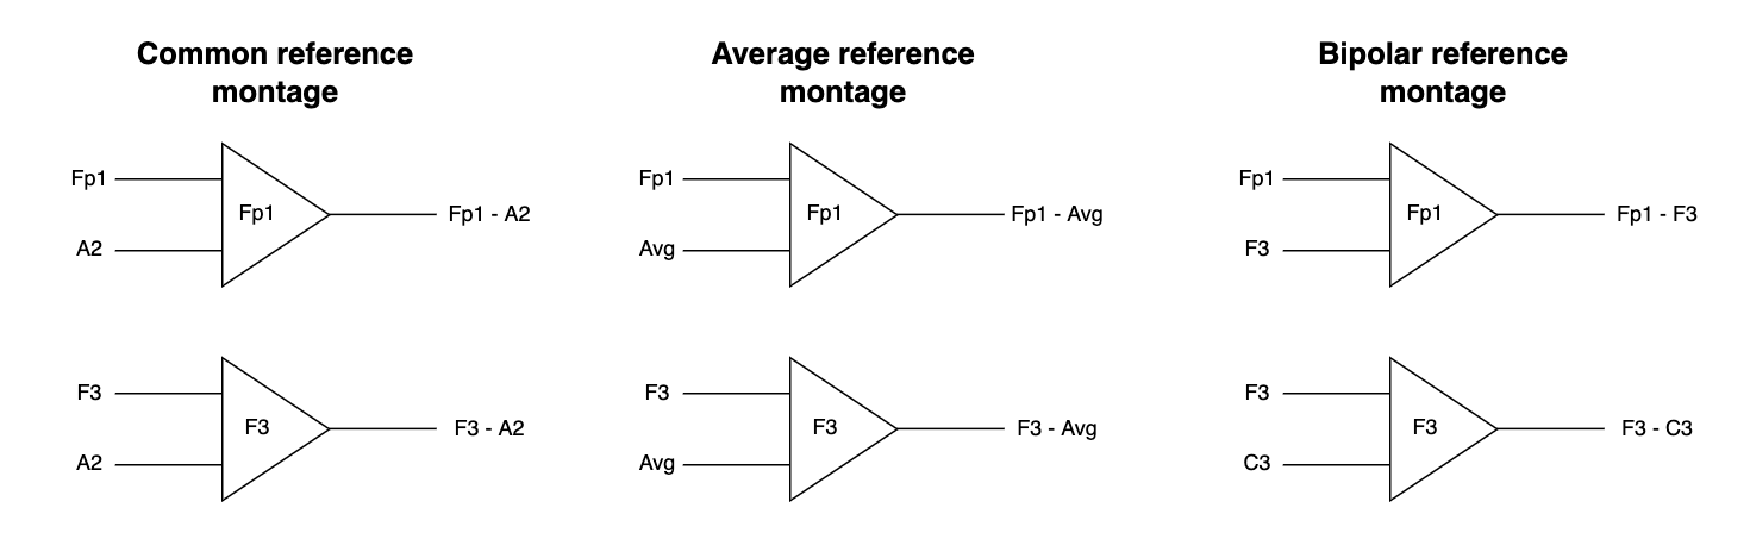
\includegraphics[width=\linewidth]{../images/eeg/montages.pdf}
    \captionsetup{width=0.8\linewidth}
    \captionsetup{justification=centering}
    \caption{Illustration of the three most common montages for the differential amplifier in EEG. The annotations are the electrode names used in the international 10–20 system.} 
    \label{fig:biomedical_signals_eeg_montages}
\end{figure}

\Gls{eeg} is one of the most popular neuroimaging modalities and also the most common modality in \gls{bci} research \citep{modalities_review1, modalities_review2, bci_review_arnau}.
This success is due to the good temporal resolution, its non-invasive nature and the relatively low cost of \gls{eeg} hardware, further discussed in Section \ref{subsec:biomedical_signals_measuring_brain_equipment}.
Many different types of headsets and caps exist which hold the electrodes in place and with minimal modification, these headsets are easy to install and use, which is also an attractive property of \gls{eeg}.

However, some of the headsets for dry electrodes, such as the Ultracortex Mark IV discussed in Section \ref{subsec:bci_opportunities_obstacles_motivating_examples}, can be unpleasant to wear over prolonged sessions.
Other disadvantages include the poor spatial resolution as discussed in Section \ref{subsec:bci_gaining_popularity_better_measuring}.
This poor spatial resolution combined with multiple fluids and structures blocking the electrical signals coming from the brain means that the data collected from \gls{eeg} is relatively low in quality, both from a \gls{snr} perspective and a source localisation perspective.
Since \gls{eeg} measurements are limited to the activity of neurons in the grey matter, not all brain activity can be measured by \gls{eeg} either.
Section \ref{subsec:biomedical_signals_biosignals_electrical} and \citet{what_eeg_is_and_measures} explain in greater detail what \gls{eeg} effectively measures.
Some studies have also shown that extensive \gls{eeg} use can cause temporary hair loss and the electrolytic gel could also cause allergic effects for the user \citep{eeg_hair_loss, dry_electrode_status}.




% | | | | | | | | | | | | |

\subsubsection{Electrocorticography (ECoG)}
\label{subsubsec:biomedical_signals_measuring_brain_modalities_ecog}

% TODO: start here

% invasive EEG
% ecog: Modalities include the electrocorticogram where electrodes are implanted on the top of the cortex, right under the skull. There is also the possibility to implant electrodes directly in the brain matter (intracortical EEG) to further increase SNR and spatial resolution. However, such invasive approaches fall outside of the scope of this article.


% | | | | | | | | | | | | |

\subsubsection{Intravescular electrodes}
\label{subsubsec:biomedical_signals_measuring_brain_modalities_intravesc_electrodes}


% | | | | | | | | | | | | |

\subsubsection{Functional near-infrared spectroscopy (fNIRS)}
\label{subsubsec:biomedical_signals_measuring_brain_modalities_fnirs}

% | | | | | | | | | | | | |

\subsubsection{Other modalities}
\label{subsubsec:biomedical_signals_measuring_brain_modalities_others}

% ook deze heel invasive vermelden? https://en.wikipedia.org/wiki/Intracortical_encephalogram_signal_analysis

% Alternative signals include magnetoencephalogram (Gross 2019), functional near infrared spectroscopy (Naseer and Hong 2015), and functional Magnetic Resonance Imaging (Sitaram et al 2007). Lesser known signal types are also becoming usable, such as acoustic resonance (Norman et al 2021), which uses the Doppler effect to detect changes in brain activity, and Photoplethysmogram (Han et al 2020), which uses optical reflections to monitor brain activity, in a similar way to near infrared spectroscopy. Another possibility is to monitor spinal cord activity using magnetospinography (Sakakiet al 2020) if one is only interested in lower-limb activity
% UIT bci_review_arnau

% The technique of MRS or magnetic resonance spectroscopy can measure something closer to action potentials but it too has issues and has not gained wide usage. It has enormous potential and hopefully will become integrated into the toolbox of neuroimagers

% - - - - - - - - - -
% Why EEG
% - - - - - - - - - -

\subsection{EEG is the most common measuring modality in BCIs}
\label{subsec:biomedical_signals_measuring_brain_why_eeg}

% bci_invasive_or_not1
% bci_invasive_or_not2


% - - - - - - - - - -
% EEG standards
% - - - - - - - - - -

\subsection{Standards for EEG measuring systems}
\label{subsec:biomedical_signals_measuring_brain_standards}

% The international 10 20 systems is a standard method of measuring the head and placing electrodeS. Depends on four main components of the head that are easily transfarable between patients, first is the nasion at the bridge of the nose then the inion at the back of the head and then two pre-auricular points near the ear
% https://www.youtube.com/watch?v=XMizSSOejg0 

% To ensure consistent electrode placement it is often the case that the standardised ‘10/20’ system is implemented (Jasper, 1958). The values 10 and 20 indicate that the distances between adjacent electrodes are either 10 % or 20 % of the total front-back or right-left size of the skull. Figure 2.1a gives a graphical representation of the standardised ‘10/20’ system. The labels of the electrodes relate to the lobes of the brain for which they record. With the advancement of EEG electrodes, various extensions of the standardised ‘10/20’ system have emerged. Figure 2.1b gives a graphical representation of the ‘10/10’ system (Oostenveld & Praamstra, 2001). For a detailed review of a range of electrode placement schemes, the reader is referred to the work of Jurcak et al. (2007).
\lipsum[1-2]

% - - - - - - - - - -
% available equipment
% - - - - - - - - - -

\subsection{Comparison of available EEG measuring equipment}
\label{subsec:biomedical_signals_measuring_brain_equipment}

% There is a wide variety in the devices used for the acquisition of each signal. For EEG, the number of recorded channels (electrodes) varies from a single channel to 64 channels, with sampling frequencies ranging from 128 to 1000 Hz. For the types of electrodes used, there is no dominating type with both wet and dry, and active and passive electrodes being
% Uit Arnau?

Many comparisons between different types of measuring equipment, often with greatly differing costs, have already been made \citep{bci_cheap_viability1, bci_cheap_viability2, bci_cheap_viability3, bci_cheap_viability4, bci_cheap_viability5}.
The main consensus is that the cheaper consumer-grade equipment has the potential to reach similar performance of a conventional, often medical-grade, BCI system.
These results are promising but due to the controlled nature of the experiments, they might not reflect real-life applications accurately.
As discussed before, the user experience of a \gls{bci} system is as important if not more important then the raw performance of the system.
% FROM: cheap_bci_feasibility
% OpenBCI1 is an open-source, versatile and affordable biosensing system which can be used to acquire not only EEG signals but also to measure electrical activity of muscle (EMG) and heart (ECG). All OpenBCI boards are based on the open-source electronic platform Arduino with wireless connection to the computer. OpenBCI offers a variety of low-cost amplifiers (boards), electrode systems (e.g. 3D-printed headware) and a software for viewing and recording the biosignals (OpenBCI GUI).2
% as well as from the user’s comfort perspective [4, 13, 14].

% TODO: Different affordable consumer-grade EEG devices have appeared in both Academia (e.g. [5, 6, 7, 8]) and the market (e.g. B-Alert X10, NeuroSky, OpenBCI, Emotiv)
% FROM: cheap_bci_feasibility

% TODO
todo
\lipsum[1-7]

% https://imotions.com/blog/eeg-headset-prices/
% Nextmind 
% Neurosky
% Interaxon
% Muse
% Emotiv
% myBrain
% OpenBCI
% Emotiv EPOC headset

% TODO: citing for sources of img?
% this image was here: https://docs.google.com/document/d/1uaRHNNBJsR8vqT50TllE8s3Jf2dUtAVCcLJb-vhncMM/edit

% - - - - - - - - - -
% artefacts
% - - - - - - - - - -

\subsection{Common EEG artefacts}
\label{subsec:biomedical_signals_measuring_brain_artefacts}

% TODO also discuss how to use them e.g. eye blink as input, ook bespreken niet goed voor e.g. sroke patienten
\lipsum[1-5]

% ---------------------------------------------- 
% WORKING WITH EEG
% ---------------------------------------------- 

% TODO: start here
% TODO 'bci paradigms" 
% info about signals: https://www.e-iji.net/dosyalar/iji_2021_2_48.pdf

\section{Working with EEG}
\label{sec:biomedical_signals_working_with_eeg}

% \gls{elecbiosignal}
\lipsum[1-2]


% - - - - - - - - - -
% anatomy
% - - - - - - - - - -

\subsection{Anatomy of the brain}
\label{subsec:biomedical_signals_working_with_eeg_anatomy}
% Bespreken welke regions important voor MI
% al getoond in bci chapter

\lipsum[1-2]

% - - - - - - - - - -
% Brain waves
% - - - - - - - - - -

\subsection{The five widely recognized brain waves}
\label{subsec:biomedical_signals_working_with_eeg_brain_waves}
% table wolf
% 2.1.1 Brain Waves from https://www.sciencedirect.com/book/9780128044902/introduction-to-eeg-and-speech-based-emotion-recognition
% bespreken hoe frequentie belangrijk en dus vaak frequency analysis en ook bespreken range MI

\lipsum[1-3]

% - - - - - - - - - -
% Measurable brain activity
% - - - - - - - - - -

\subsection{Common brain signal inducing methods}
\label{subsec:biomedical_signals_working_with_eeg_inducing_methods}

% bci_applications heeft ook overview onder 6. BCI electrical signal

% Since these signals can capture neural activity related to sensory and cognitive processes, they are called Event-Related Potentials (ERP). Examples of ERPs are Slow Cortical Potentials (SCP; Kleber & Birbaumer, 2005), which are very slow fluctuations in cortical activity that can be made positive or negative through operant conditioning, ERrorRelated Potentials (ErrP; Abiri et al., 2019), which occur when a BCIs action does not correspond with the user’s intention, Steady-State Evoked Potentials (SSEP; Djamal & Lodaya, 2017), which appear when a person perceives a periodic stimulus, and Movement Related Cortical Potentials (MRCP; Shakeel et al., 2015), which are low-frequency negative shifts that take place about 2 seconds prior to voluntary movement. An overview of ERPs and their usage in BCIs is described by Rashid et al. (2020).

% it is important to note that a person’s intention can not only be decoded from invoked potentials such as ERPs but also from phenomena such as Event-Related Synchronisation (ERS) and Event-Related Desynchronisation (ERD). These denote, respectively, the increase and decrease of oscillatory activity within frequency bands (Pfurtscheller & da Silva, 2017). Such oscillations are known to occur in preparation for movement or imagining movement, i.e., motor imagery. Certain body parts, like the hands and tongue, are associated with a large and distinguishable cortical area, which has allowed BCIs to control them via motor imagery (Schl¨ogl et al., 2005).

% TODO
% echt uitleggen wat ERP is
% ssvep
% p300 zeker
% MI
% erd

\lipsum[1-7]

% TODO zie chapter 23 bci_handbook
% Issues MI: https://www.frontiersin.org/articles/10.3389/fnins.2021.824759/full
\Gls{mi} is the process in which a person generates brain-activity in the motor cortex merely by imagining motor movements.
\Gls{mi}-based \glspl{bci} are interesting because they don't require any external stimulus nor effective motor movements

\glspl{erp} and the measurable signals they produce, such as the P300 signal, are only one of many sources for detectable brain signals.
In general, \gls{erp} related signals are easier to detect reliably, as the stimulus can be controlled, giving a hint when and where to look for signals and what to look for.

An alternative to \glspl{erp} is using a mental phenomenon called \gls{mi} as source of signals for a \gls{bci} system.
\Gls{mi} is the process in which a person generates brain activity in the motor cortex merely by imagining motor movements.
Section \ref{subsec:biomedical_signals_working_with_eeg_inducing_methods} explains in further detail how \gls{mi} is not dependent on an external stimuli nor actual motor movements.
This makes \gls{mi}-based \glspl{bci} extra appealing as they don't require external stimuli and are applicable for people with motor disabilities.
\Citet{first_mi} were the first to experiment with the idea of using \gls{mi} in an \gls{eeg} classification task.
Since then, many \gls{mi}-based \glspl{bci} have been proposed.
% MI can be trained

% - - - - - - - - - -
% generalisation issues
% - - - - - - - - - -

\subsection{Generalisation issues of brain activity}
\label{subsec:biomedical_signals_working_with_eeg_generalisation}

% neuroplasticity and inter-human variation en non stationarity en mapping brain en... bespreken

% However, as mentioned, since this is an invasive technique, it is not discussed here. Lastly, a crucial property of EEG in the context of machine learning, is its nonstationarity (Klonowski, 2009). A stationary signal is one of which the properties do not change with time. On the other hand, a nonstationary signal is inconsistent with time. EEG’s nonstationarity is a result of it capturing the activity of a multitude of different latent variables in the brain, each of which are transmitting with different and variable intensity. In a fraction of a second, the latent variables whose activities are currently dominant can change. Nonstationarity makes interpreting EEG a nontrivial task. If not properly addressed, machine learning models are certain to struggle to learn anything valuable from EEG. This is reflected by the number of preprocessing and feature extraction methods that exist for EEG.

\lipsum[1-3]


% ---------------------------------------------- 
% CONCLUSIONS OF CHAPTER
% ---------------------------------------------- 
\section{Motivation for using non-invasive MI EEG and chapter conclusions}
\label{sec:biomedical_signals_summary}
% TODO: summary of this chapter

% uitleggen waarom EEG en MI

% uitleggen dat hybrid in de toekomst mss wel beter zal zijn maar momenteel nog geen zicht op

\lipsum[1-3]